%! TeX program = lualatex
\documentclass[main]{subfiles}

\begin{document}

\title[AutoML: HPO]{Big Picture}
\subtitle{The Importance of Hyperparameters}
\author[Lars Kotthoff]{Lars Kotthoff}
\date{}

%\institute{}
%\date{}

	\maketitle
	

\begin{frame}{Introduction}
    \begin{itemize}
        \item Training ML models fits (``learns'') parameters to the data (e.g.\ coefficients of a polynomial)
        \item Hyperparameters specify what parameters should be learned and how this learning should be done
        \item Examples of hyperparameters: number of trees in a random forest, learning rate in a neural network, kernel in a Gaussian process
    \end{itemize}
\end{frame}

%----------------------------------------------------------------------

\begin{frame}{Motivating Example}
    \begin{columns}
        \column{.5\textwidth}
        XGBoost on OpenML dataset 11 (balance-scale)
        \begin{itemize}
            \item default hyperparameters: 75.87\% ±8.1\% accuracy
            \item ``gblinear'' booster: 85.45\% ±5.6\% accuracy
        \end{itemize}
        $\leadsto$ 10\% accuracy improvement with simple hyperparameter change

        \column{.5\textwidth}
        \begin{center}
            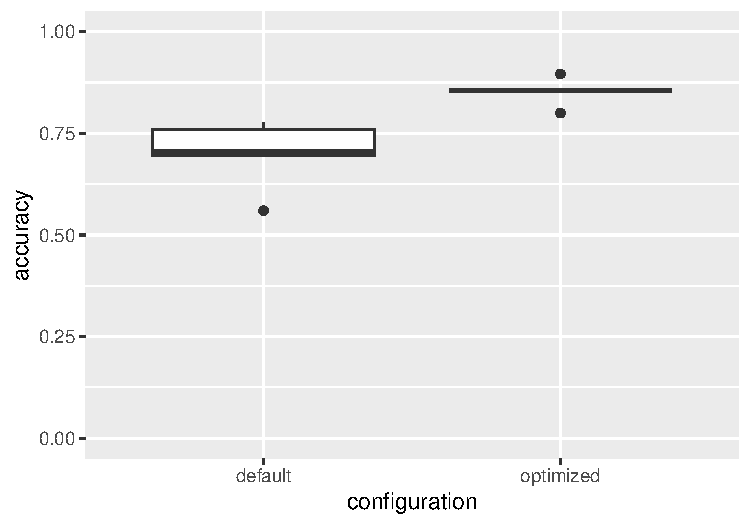
\includegraphics[width=\textwidth]{images/mot}
        \end{center}
    \end{columns}
\end{frame}

%----------------------------------------------------------------------

\begin{frame}{Hyperparameters}
    \begin{itemize}
        \item Hyperparameters have to be set in every ML application
        \item They systematically and semantically affect what is learned and how
        \item \emph{Not} merely options of an implementation -- it makes no sense to tune e.g.\ random seed, debug output level, or number of jobs to optimize model performance
        \item We call a complete set of values for each hyperparameter a \emph{configuration}
        \item Without a configuration, we cannot train ML models
        \item A configuration, or part of one, could be the \emph{default}, i.e.\ we do not explicitly set values, but rely on values that the provider of the ML system has chosen
    \end{itemize}
\end{frame}

%----------------------------------------------------------------------

\begin{frame}{Hyperparameter Optimization}
    \begin{itemize}
        \item Default configurations often allow to train models with reasonable performance (hopefully!), but usually not the best performance
        \item \emph{Hyperparameter Optimization} is the (systematic) search through the space of possible configurations for the best-performing one
        \item Can yield substantial performance improvements that make a difference in practice
    \end{itemize}
    
    $$\optconf \in \argmin_{\conf \in \pcs} \riskg(\mathcal{I}(\datasettrain, \conf) \mid \datasetval)$$
\end{frame}

%----------------------------------------------------------------------

\begin{frame}{Summary} 
\begin{enumerate}
    \item Hyperparameters control what model parameters the ML training process fits and how
    \item Default hyperparameter configurations often perform well
    \item \ldots{}but for the best performance, configurations should be optimized to the given task, as the performance of configurations varies across tasks
\end{enumerate}
\end{frame}

\end{document}
